\section{Výkon na reálných datech}
\label{sec:Chapter52}
Model YOLOv11-s použitý pro lokalizaci objektu Hot Rod 42022 v kombinaci s metodou řešení perspektivního problému $n$ bodů \texttt{cv2.SOLVEPNP\_ITERATIVE} a robustní metodou RANSAC dosáhl uspokojivých výsledků. Při testování na videosekvencích se osvědčil jak samotný detekční model, tak i následný odhad pózy. Za předpokladu správné kalibrace kamery a odpovídajícího nastavení kamerové matice přístup poskytuje přesné a stabilní výsledky. Při testování volby \texttt{useExtrinsicGuess} ve spojení s předchozími hodnotami vektorů \texttt{tvec} a \texttt{rvec} během zpracování videosekvence nebyl pozorován žádný rozdíl ve výsledcích.

Za pozoruhodné omezení lze považovat sníženou přesnost lokalizace klíčových bodů v případech, kdy objekt není plně zachycen v záběru -- a to i přesto, že podobné situace jsou v trénovacím datasetu poměrně hojně zastoupeny. Naopak odhad ohraničujícího boxu je ve většině případů spolehlivý. U vzdálenějších záběrů modelu auta byl v krajních případech zaznamenán nepřesný odhad pózy, což lze pravděpodobně přičíst nedostatečnému zastoupení takových snímků v trénovací množině.

\begin{figure}[ht]
\centering
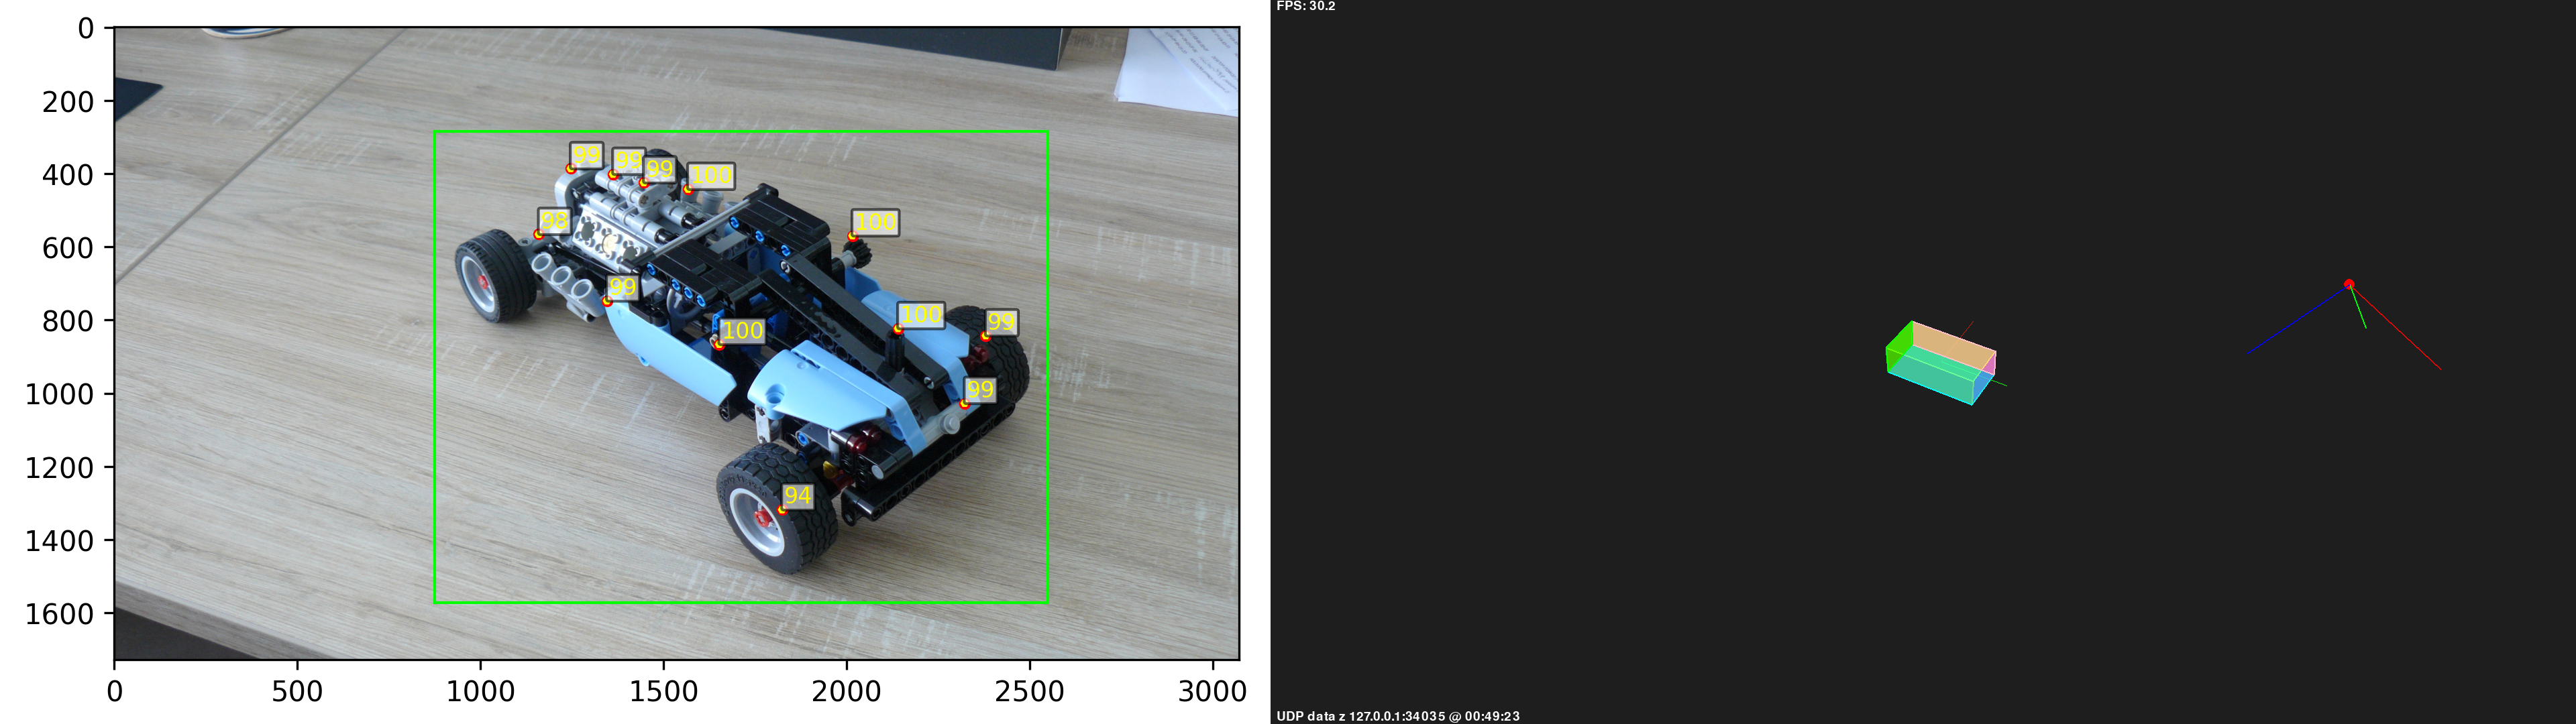
\includegraphics[width=1.0\textwidth,keepaspectratio]{Figures/pnp.png}
\caption[Odhad pózy modelu Hot Rod 42022]{Odhad pózy modelu Hot Rod 42022}
\label{fig:pnp}
\end{figure}

\begin{figure}[ht]
\centering
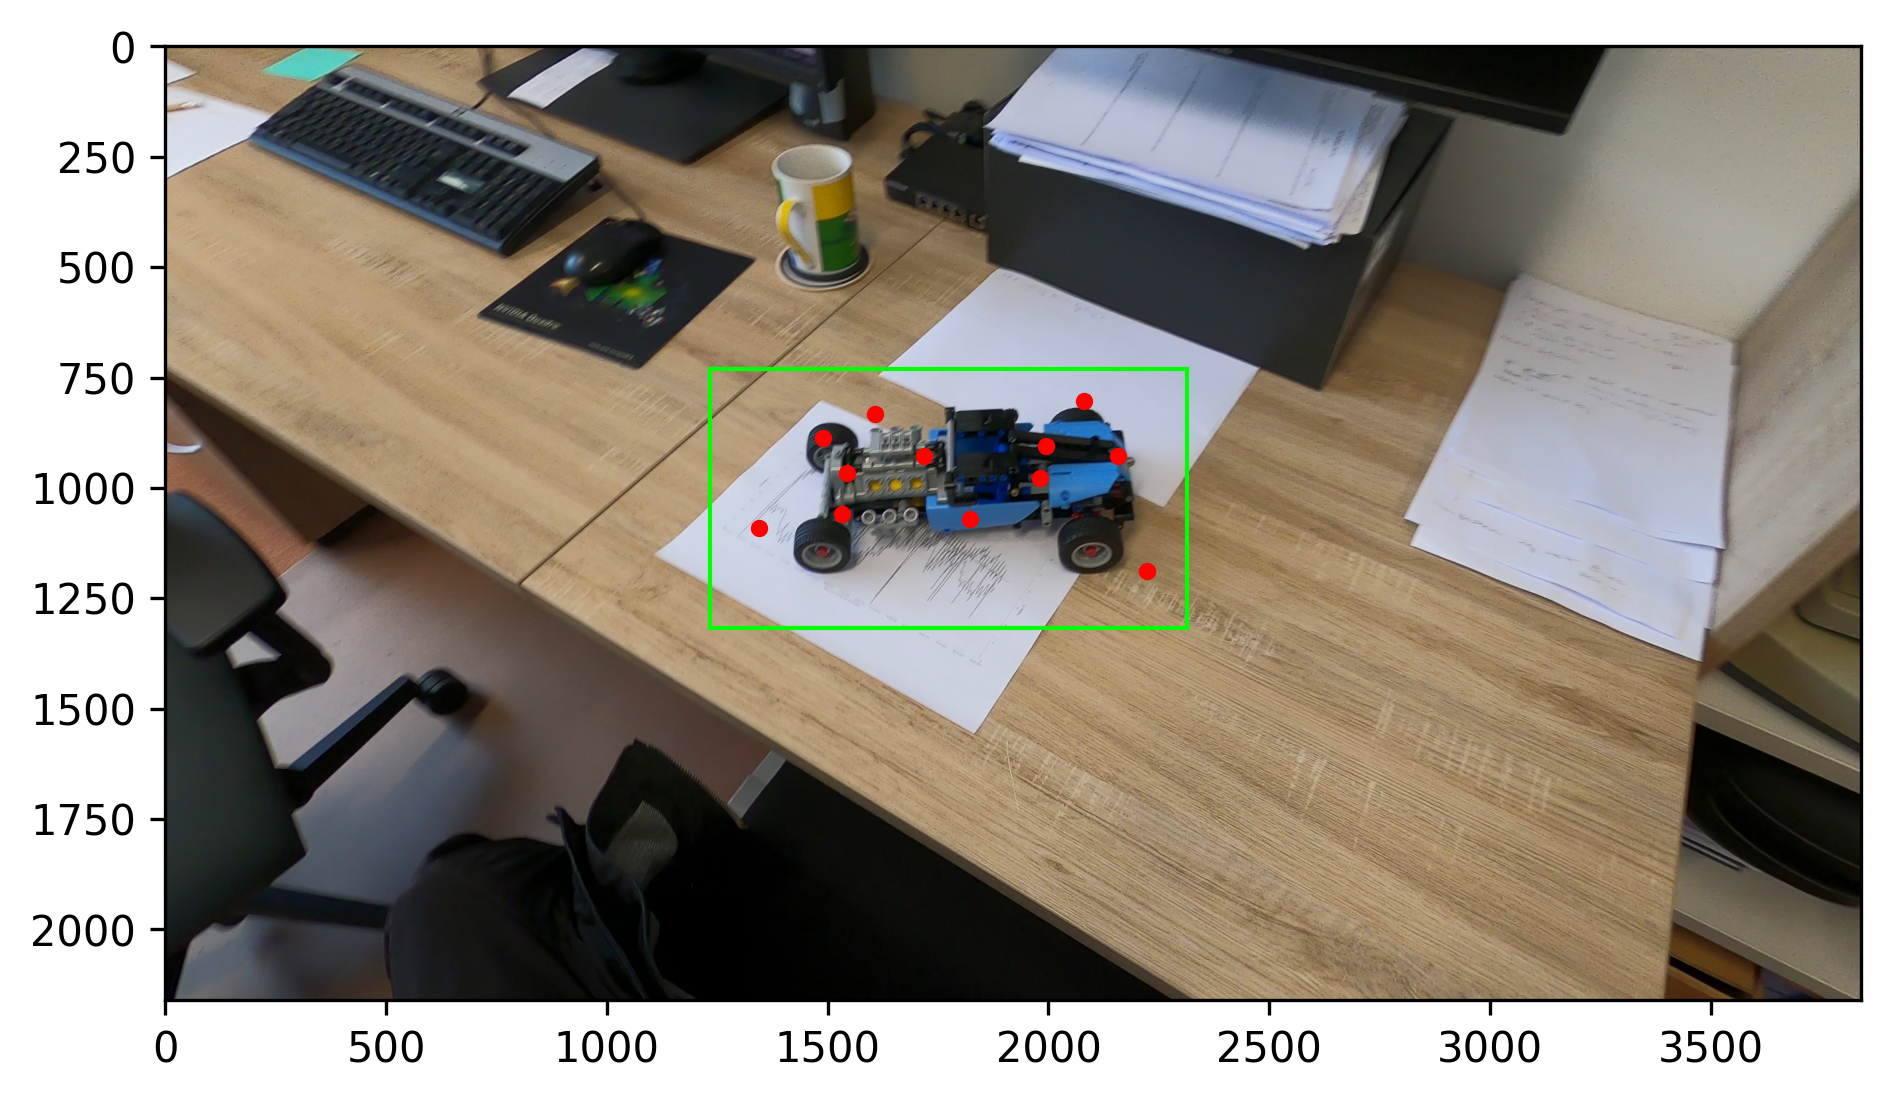
\includegraphics[width=0.7\textwidth,keepaspectratio]{Figures/nepresny.png}
\caption{Nepřesný odhadu pózy modelu Hot Rod 42022}
\label{fig:inaccurate}
\end{figure}